\section{Vermaschte Regelkreise}


\subsection{Allgemeines}

Die in Bild \ref{fig:7-1} wiedergegebene Struktur des Einfachregelkreises lässt sich unter bestimmten Umständen durch zusätzlich einzuführende Wirkungslinien und Übertragungsglieder wesentlich verbessern.

\begin{figure}[ht]
    \centering
    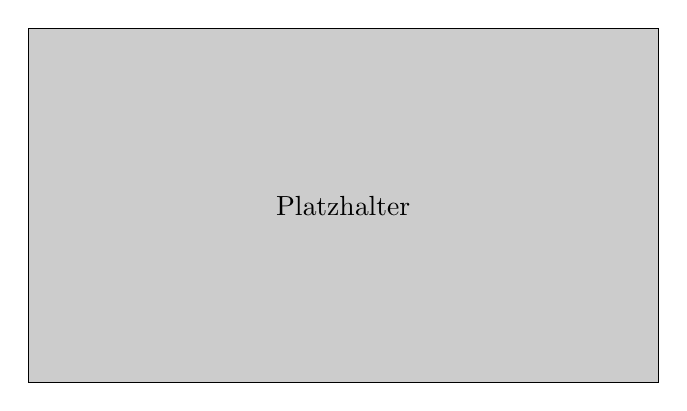
\begin{tikzpicture}
        \filldraw[fill=white!80!black,draw=black] (0,0) rectangle (8,4.5) node[pos=.5] {Platzhalter};
    \end{tikzpicture}
    \caption{Einfacher Regelkreis}
    \label{fig:7-1}
\end{figure}

Im Folgenden sollen einige Maßnahmen erläutert werden, die in vielen Fällen zu Regelungssystemen mit deutlich besseren Eigenschaften führen, als sie der Einfachregelkreis aufweist.
Diese Maßnahmen sind i. Allg. nur unter bestimmten Voraussetzungen anwendbar und bedingen fast immer einen zusätzlichen Geräteaufwand, der die Regelungseinrichtung verteuert.
Andererseits sind sehr viele technische Prozesse mit einer einschleifigen Regelung überhaupt nicht oder nicht mit der erforderlichen Genauigkeit zu regeln.

Neben den vorzustellenden Maßnahmen
\begin{itemize}
	\item Vorregelung der Störgrößen,
	\item Aufschalten von Hilfsstellgrößen,
	\item Aufschalten von Hilfsregelgrößen,
	\item Kaskadenregelung,
	\item Vorsteuerung,
	\item Führungsgrößenfilter und
	\item Mehrgrößenregelung
\end{itemize}
gibt es zahlreiche andere, die z. T. Mischformen der erwähnten darstellen.
Die technischen Gegebenheiten sind so vielfältig, dass die folgende Darstellung nur als Orientierungshilfe aufgefasst werden kann.
Anschließend wird in diesem Kapitel auf einige Besonderheiten der Mehrgrößen-Regelung eingegangen.


\subsection{Vorregelung}

Vorregelungen haben die Aufgabe, Störungen des zu regelnden Prozesses so weit wie möglich zu verringern, indem Einflussgrößen, deren Änderungen störend wirken, durch zusätzliche, meist sehr einfach aufgebaute Regelungen konstant oder nahezu konstant gehalten werden.

Bild \ref{fig:7-2} zeigt den Wirkungsplan eines Regelkreises mit Vorregelung, die aus der Regelstrecke \(S_v\) und dem Regler \(R_v\) besteht.
Die Vorregelung soll die Störgröße \(z\) verringern, sodass nur noch die verminderte Störgröße \(z'\) auf den Hauptregelkreis einwirkt.
Es leuchtet ein, dass die durch die Vorregelung zu vermindernden Störgrößen messbar und beeinflussbar sein müssen.

\begin{figure}[ht]
    \centering
    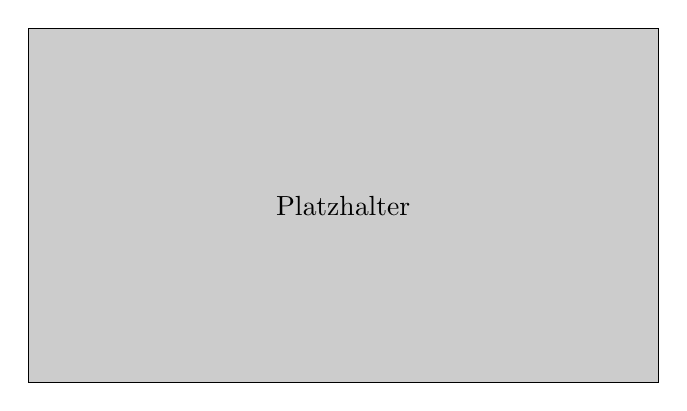
\begin{tikzpicture}
        \filldraw[fill=white!80!black,draw=black] (0,0) rectangle (8,4.5) node[pos=.5] {Platzhalter};
    \end{tikzpicture}
    \caption{Vorregelung}
    \label{fig:7-2}
\end{figure}

Als Beispiel möge die Vorregelung des Gasdruckes an gasbeheizten Öfen dienen.
In Bild \ref{fig:7-2} entspricht die Störgröße \(z\) den Druckschwankungen im Versorgungsnetz, die durch einen Druckregler \(S_v\), \(R_v\) vermindert werden, sodass ihr Einfluss auf die Ofentemperatur \(x\) gering bleibt.
Weil die Temperatur noch durch andere Einflüsse verändert werrden kann, die sich einer Vorregelung entziehen, kann man auf den Hauptregler \(R\) nicht verzichten.
Als Vorregler wird of ein einfacher Druckregler ohne Hilfsenergie eingesetzt.

Eine Vorregelung verbessert nicht nur das Störverhalten von Regelungen bezüglich der durch die Vorregelung erfassten Störgrößen, in vielen Fällen trägt sie auch dazu bei, dass der notwendige Stellbereich, der vom Hauptregler beeinflussten Stellgröße (\(y\) in Bild \ref{fig:7-2}), verringert werden kann, was oft die Wirtschaftlichkeit des gesamten Prozesses verbessert.


\subsection{Störgrößenaufschaltung}

Durch die Störgrößenaufschaltung werden aus der Änderung von Größen, die den zu regelnden Prozess stören, zweckmäßige Änderungen der Stellgröße des Hauptregelkreises abgeleitet.
Die Stellgröße kann im Idealfall die Wirkung der Störung genau kompensieren, sodass die Regelgröße durch diese Störung nicht beeinflusst wird.

Wie Bild \ref{fig:7-3} zeigt, wird die Störgröße \(z\) gemessen und durch das Aufschaltgerät \(A\) der vom Regler erzeugten Stellgröße überlagert.
Man erkennt, dass für
\begin{equation}
	G_A = 1
\end{equation}
duie resultierende Stellgrößenänderung die Störgröße \(z\) vollständig kompensieren würde.

\begin{figure}[ht]
    \centering
    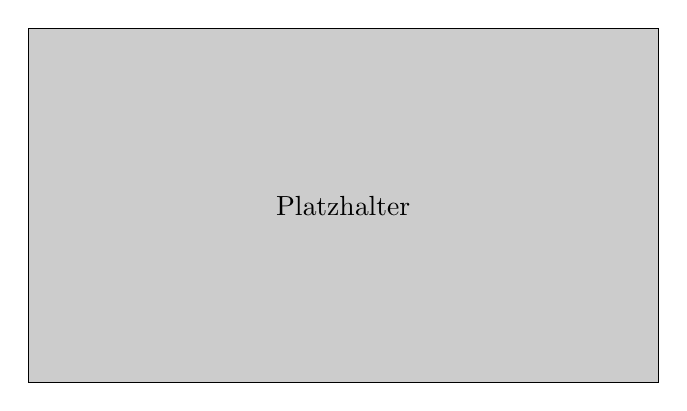
\begin{tikzpicture}
        \filldraw[fill=white!80!black,draw=black] (0,0) rectangle (8,4.5) node[pos=.5] {Platzhalter};
    \end{tikzpicture}
    \caption{Störgrößenaufschaltung}
    \label{fig:7-3}
\end{figure}

Bei Regelungen mit analogen Einzelgeräten wird häufig die im folgenden Bild \ref{fig:7-4} dargestellte Struktur benutzt, bei der die Störgröße auf die Regelabweichung aufgeschaltet wird.
Die Wirkung beider Aufschaltungen ist gleich, wenn in Bild \ref{fig:7-4} zur vollständigen Kompensation
\begin{equation}
	G_A \cdot G_R = 1
\end{equation}
gesetzt wird und damit
\begin{equation}
	G_A = \frac{1}{G_R}
\end{equation}
wird.
Für die Struktur nach Bild \ref{fig:7-4} sprechen vielfach die geringeren Gerätekosten; dies gilt nicht, wenn die Aufschaltung z.B. innerhalb von digitalen Prozessleitsystemen oder ähnlichen Rechnern verwirklicht wird.

\begin{figure}[ht]
    \centering
    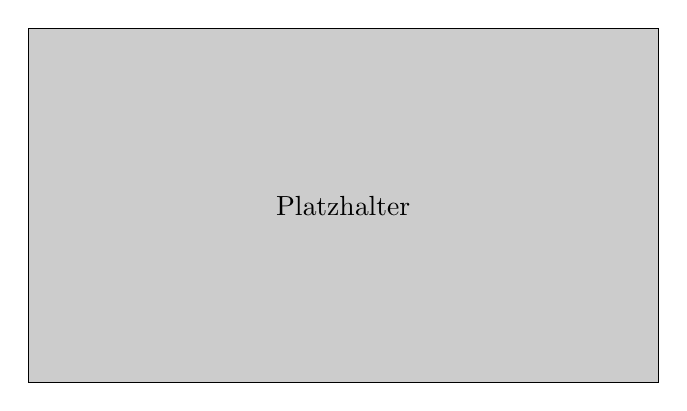
\begin{tikzpicture}
        \filldraw[fill=white!80!black,draw=black] (0,0) rectangle (8,4.5) node[pos=.5] {Platzhalter};
    \end{tikzpicture}
    \caption{Störgrößenaufschaltung}
    \label{fig:7-4}
\end{figure}

Bei Reglern mit integrierendem Verhalten ist es wichtig, dass das Aufschaltgerät bei zeitlich konstanter Störgröße \(z\) eine in angemessener Zeit verschwindende Ausgangsgröße abgibt, weil sonst die Regelgröße nicht der Führungsgröße angeglichen wird.
Z. B. muss für einen Hauptregler mit \(PI\)-Verhalten ein Aufschaltgerät mit nachgebendem Verhalten eingesetzt werden.

Störgrößenaufschaltungen sind dann zweckmäßig, wenn der zu regelnde Prozess durch wenige gut messbare Störgrößen beeinflusst wird und eine Vorregelung dieser Größen nicht möglich oder nicht wirtschaftlich ist.
Eine wesentliche Verbesserung gegenüber einer einfachen Regelung kann man dann erwarten, wenn die Regelstrecke Totzeitglieder enthält, die bekanntlich eine wirksame Regelung erschweren, und die aufzuschaltende Störgröße ebenfalls über diese Totzeitglieder auf die Regelgröße wirkt.
Im Gegensatz dazu bringt die Aufschaltung einer Störgröße, die sich ohne wesentliche Verzögerung additiv auf die Regelgröße auswirkt (\(z_1\) in Bild \ref{fig:7-4}), i. Allg. keine Verbesserung.

Aus den Bildern \ref{fig:7-3} und \ref{fig:7-4} ist zu erkennen, dass die Störgrößenaufschaltung eine reine Steuerung ist.
Daher sind mit dieser Maßnahme keine Stabilitätsprobleme verbunden.
Der Erfolg einer solchen Maßnahme hängt andererseits wesentlich von der richtigen Abstimmung dieser Steuerung ab.

Ein weit verbreitetes Anwendungsbeispiel für Störgrößenaufschaltungen ist die Veränderung der Vorlauftemperatur in Zentralheizungsanlagen als Funktion von Änderungen der Außentemperatur.
Bei Raumtemperaturregelungen ist die Außentemperatur eine der wichtigsten Störgrößen.
Wenn durch geeignete Steuerung der Temperatur des Heizungsvorlaufs die Wirkung von Außentemperaturschwankungen auf die Raumtemperatur ganz oder teilweise angeglichen wird, so kann der Raumtemperaturregler i. Allg. einfacher und damit billiger sein und seine Aufgabe dennoch besser erfüllen als ein Regler in einem einfachen Regelkreis.


\subsection{Hilfsstellgröße}

Wenn der zu regelnde Prozess im Wirkungsplan als Reihenschaltung mehrerer Verzögerungsglieder darstellbar ist (Bild \ref{fig:7-5}), so kann es sinnvoll sein, eine zusätzliche Stellgröße, die Hilfsstellgröße \(y_h\), zu verwenden.
Wichtigste Voraussetzung dafür ist, dass eine solche Stellgröße überhaupt in die Regelstrecke eingeführt werden kann.

\begin{figure}[ht]
    \centering
    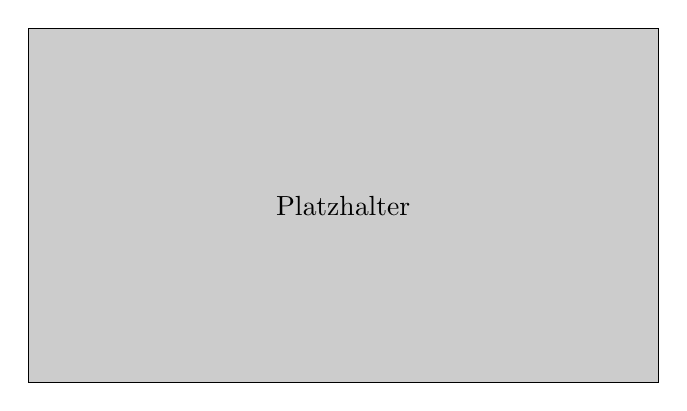
\begin{tikzpicture}
        \filldraw[fill=white!80!black,draw=black] (0,0) rectangle (8,4.5) node[pos=.5] {Platzhalter};
    \end{tikzpicture}
    \caption{Aufschaltung einer Hilfsstellgröße}
    \label{fig:7-5}
\end{figure}

Die Hilfsstellgröße und der sie erzeugende Regler \(R_h\) bilden mit einem Teil der Regelstrecke einen Unterregelkreis.
Dieser kann i. Allg. wesentlich günstigere dynamische Eigenschaften haben als der Hauptregelkreis, weil die zugehörige Teilregelstrecke von niedrigerer Ordnung ist als die zum Hauptregelkreis gehörende Regelstrecke und der Hilfsregler \(R_h\) daher entsprechend schneller arbeiten kann.

Weil der Unterregelkreis die gleiche Führungsgröße und die gleiche Regelgröße wie der Hauptregelkreis verarbeitet und dies unter günstigeren Bedingungen für gute Dynamik tut, könnte man meinen, der Hauptregelkreis sei überflüssig.
In der technischen Wirklichkeit ist dieser Schluss meist falsch, weil z. B. die Hilfsstellgröße einen so kleinen Stellbereich hat, dass sie allgemein nicht alle Störungen ausgleichen kann oder wiel sie als alleinige Stellgröße unwirtschaftlich wäre.
Aufgrund derartiger Einschränkungen werden als Hilfsregler meist solche mit \(P\)-, \(PD\)- oder nachgebendem Verhalten eingesetzt.

\begin{figure}[ht]
    \centering
    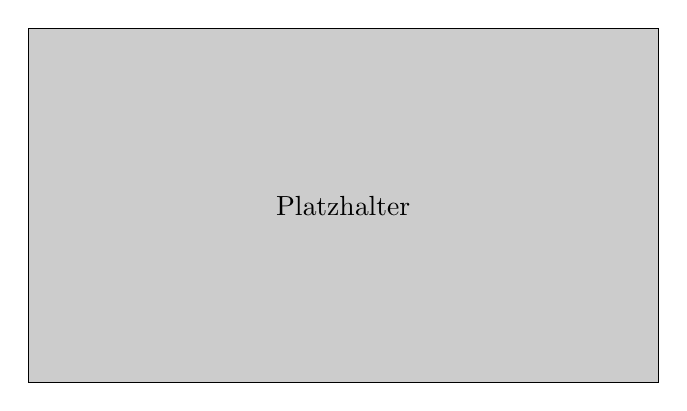
\begin{tikzpicture}
        \filldraw[fill=white!80!black,draw=black] (0,0) rectangle (8,4.5) node[pos=.5] {Platzhalter};
    \end{tikzpicture}
    \caption{Dampftemperaturregelung mit Einspritzwasserstrom als Hilfsstellgröße}
    \label{fig:7-6}
\end{figure}

Ein Anwendungsbeispiel für Regelungen mit Hilfsstellgrößen zeigt Bild \ref{fig:7-6}.
Die Temperatur des von einem Dampferzeugermit Überhitzer abgegebenen Dampfes wird durch die Brennstoffzufuhr beeinflusst.
Um jedoch kurzzeitige Schwankungen der Temperatur besser ausgleichen zu können, werden nach einzelnen Überhitzern oder Überhitzergruppen sog. Einspritzkühler vorgesehen, in denen der Dampf durch eingespritztes Wasser gekühlt wird.
Der Einspritzwasserstrom ist hier Hilfsstellgröße; er wirkt erheblich schneller auf die Dampftemperatur als eine Brennstoffstromänderung.
Durch die Dampfkühlung wird allerdings der Gesamtwirkungsgrad des Dampferzeugers verschlechtert, sodass man i. Allg. anstrebt, möglichst wenig Einspritzwasser zu verwenden.

Durch den Unterregelkreis mit dem Hilfsregler \(R_h\) wird auch die Dynamik des Hauptregelkreises verändert, und zwar so, dass der Hauptregler auf größere Übertragungsfaktoren eingestellt werden kann, ohne dass der Regelkreis zu schwach gedämpft erscheint.
Damit wird das Stör- und Führungsverhalten des Regelkreises insgesamt verbessert.
Wenn diese Möglichkeit genutzt wird, besteht allerdings beim Ausfall der Hilfsstellgröße Gefahr für die Stabilität der Gesamtanlage.
Die Hilfsstellgröße kann dadurch ausfallen, dass zugehörige Geräte versagen, aber auch dadurch, dass sie infloge besonders großer Störungen die Grenzen ihres Stellbereichs erreichen.


\subsection{Hilfsregelgröße}

Wenn der zu regelnde Prozess im Wirkungsplan als Reihenschaltung mehrerer Verzögerungsglieder darstellbar ist und wesentliche Störgrößen in der Nähe des Angriffspunktes der Stellgröße auf die Regelstrecke einwirken, so werden die Auswirkungen solcher Störungen (\(z_1, z_2\) in Bild \ref{fig:7-7}) für den Regler nur stark verzögert messbar.
Das bedeutet zwar, dass die Störgrößenim Verlauf der Regelgröße nur sehr abgeschwächt zu bemerken sind, dies ist aber für eine effektive Regelung u. U. so nachteilig, dass eine zusätzliche, dem Prozess entnommene Messgröße, die solche Störungen weniger stark verzögert wiedergibt, Vorteile verspricht.
Diese Messgröße wird Hilfsregelgröße \(x_h\) genannt und dazu benutzt, die Stellgröße zusätzlich zu beeinflussen (Bild \ref{fig:7-7}).

Ähnlich wie bei der Aufschaltung einer Hilfsstellgröße wird auch hier ein zusätzlicher Regelkreis gebildet, der unter günstigeren Voraussetzungen für gute Dynamik aufgebaut werden kann und die Stabilitätseigenschaften auch des Hauptregelkreises verbessert.

Weil der Hilfsregler aber nicht die eigentlich interessierende Regelgröße \(x\) und die zugehörige Führungsgröße \(w\) verarbeitet, muss er so ausgelegt werden, dass er den Hauptregler nicht behindert.
Dies geschieht meist dadurch, dass der Hilfsregler mit \(P\)-, \(PD\)- oder nachgebendem Verhalten ausgestattet wird.
Bei Regelungen mit analogen Geräten wird aus Kostengründen häufig die in Bild \ref{fig:7-7}b dargestellte Lösung mit dem Hilfsregler \(R_h'\) benutzt.
Wenn
\begin{equation}
    G_{R_h'} \cdot G_R = G_{R_h}
\end{equation}
gilt, so sind beide Lösungen gleichwertig.

\begin{figure}[ht]
    \centering
    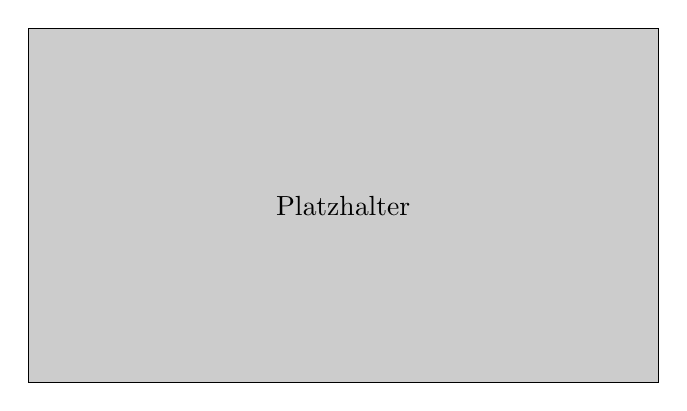
\begin{tikzpicture}
        \filldraw[fill=white!80!black,draw=black] (0,0) rectangle (8,4.5) node[pos=.5] {Platzhalter};
    \end{tikzpicture}
    \caption{Aufschaltung einer Hilfsregelgröße}
    \label{fig:7-7}
\end{figure}

Falls die Verbesserung der Dynamik des Hauptregelkreise, die durch die Hilfsregelgröße entsteht, zur Vergrößerung des Übertragungsfaktors des Hauptreglers ausgenutzt wird, ist wie im Fall der Hilfsstellgröße zu beachten, dass bei Ausfall des Hilfsregelkreises die Stabilität des Gesamtsystems gefährdet sein kann.
Wird diese Möglichkeit nicht genutzt, so vermindert der Hilfsreglernur die Auswirkungen der von ihm erfassten Störungen (\(z_1, z_2\) in Bild \ref{fig:7-7}).

Als Beispiel soll die schon einmal erwähnte Dampftemperaturregelung erneut herangezogen werden.
Entsprechend Bild \ref{fig:7-8} wird i. Allg. nicht nur die Temperatur des den Überhitzer verlassenden Dampfes gemessen, sondern auch die Temperatur des Dampfes zwischen Einspritzkühler und Überhitzer.
Diese Messgröße \(x_h\) wird zur Beeinflussung des Einspritzwasserstromes mit benutzt.

\begin{figure}[ht]
    \centering
    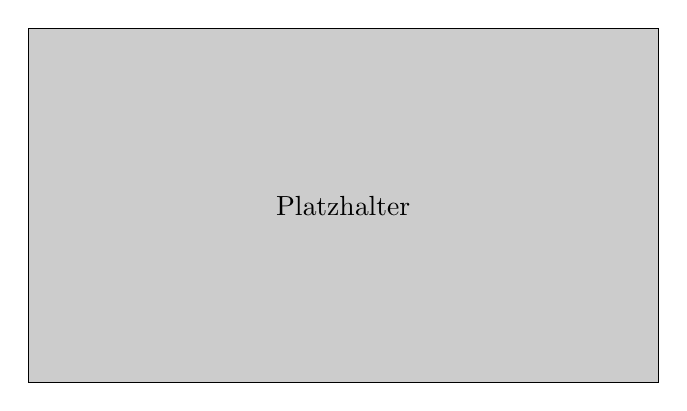
\begin{tikzpicture}
        \filldraw[fill=white!80!black,draw=black] (0,0) rectangle (8,4.5) node[pos=.5] {Platzhalter};
    \end{tikzpicture}
    \caption{Dampftemperaturregelung mit Temperatur vor Überhitzer als Hilfsregelgröße}
    \label{fig:7-8}
\end{figure}


\subsection{Kaskadenregelung}

Wenn die Voraussetzungen für den Einsatz einer Hilfsregelgröße vorliegen, so kann man Haupt- und Hilfsregler auch so anordnen, dass der Hauptregler \(R\) die Führungsgröße des Hilfreglers \(R_h\) erzeugt (Bild \ref{fig:7-9}).
Dadurch entsteht ein unterlagerter Regelkreis, in dem alle auf den vorderen Teil der Regelstrecke einwirkenden Störungen (\(z_1, z_2\) in Bild \ref{fig:7-9}) durch den Hilfsregler ausgeglichen werden.

\begin{figure}[ht]
    \centering
    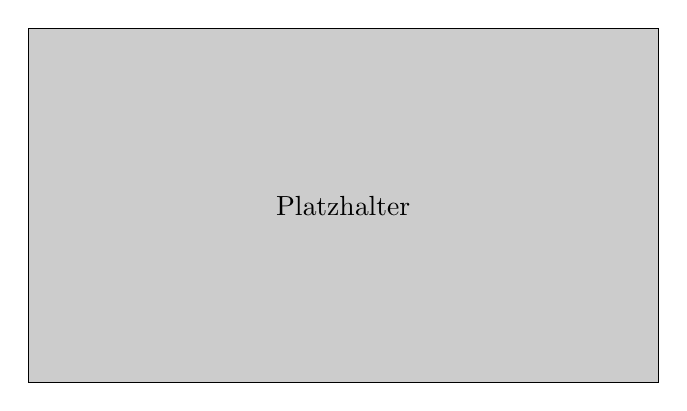
\begin{tikzpicture}
        \filldraw[fill=white!80!black,draw=black] (0,0) rectangle (8,4.5) node[pos=.5] {Platzhalter};
    \end{tikzpicture}
    \caption{Kaskadenregelung}
    \label{fig:7-9}
\end{figure}

Kaskadenregelungen sind eine sehr häufig benutzte Form vermaschter Regelkreise.
Sie werden oft nicht nur zur Verbesserung des dynamischen Verhaltens der Regelung benutzt, sondern auch um Nichtlinearitäten in einem Teil der Regelstrecke durch den Hilfsregler auszugleichen.
Unter ungünstigen Umständen können zu träge Hilfsregler die Dynamik der Gesamtanlage verschlechtern; wenn durch den Hilfsregler wesentliche Störungen wirksam gedämpft werden, kann das dennoch sinnvoll sein.

Beispiele für Kaskadenregelungen sind Regelungen in der elektrischen und hydraulischen Antriebstechnik, die oft aus mehreren ineinander geschachtelten Regelkreisen augebaut werden, um ein Gesamtsystem mit guten dynamischen Eigenschaften zu gewinnen (Bild \ref{fig:7-10}); ferner unterlagerte Stellungs- oder Mengenstromregelkreise bei verfahrenstechnischen o. ä. Anlagen sowie alle Regelungen, in denen Stellglieder mit zusätzlichen Stellungsreglern eingesetzt sind.

\begin{figure}[ht]
    \centering
    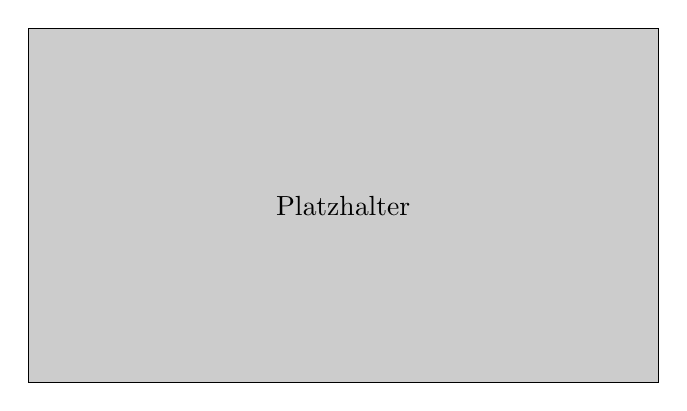
\begin{tikzpicture}
        \filldraw[fill=white!80!black,draw=black] (0,0) rectangle (8,4.5) node[pos=.5] {Platzhalter};
    \end{tikzpicture}
    \caption{Lageregelung als Kaskadenregelung}
    \label{fig:7-10}
\end{figure}

Bild \ref{fig:7-10} zeigt den Wirkungsplan einer Lageregelung mit der Regelgröße \(x\) und dem zugehörigen Hauptregler \(R\).
Dem Lageregelkreis ist ein Geschwindigkeits- (Drehzahl-)Regelkreis mit \(x_{h1}\) und \(R_{h1}\) unterlagert.
Der Geschwindigkeitsregler \(R_{h1}\) wirkt auf einen Stromregelkreis mit \(x_{h2}\) und \(R_{h2}\).
Der Stromregler \(R_{h2}\) bedient das Stellglied, das ein Thyristorstellglied sein kann.
Man erkennt, dass hier nur ein einziges Stellglied benötigt wird, aber auch, dass zum Erfassen jeder der drei Regelgrößen eine eigene Messeinrichtung vorzusehen ist.
Bei der Dimensionierung derartiger Regelkreise geht man zweckmäßigerweise von innen nach außen vor, d. h. man legt zuerst den Regler \(R_{h2}\) aus und fasst dann den mit diesem Regler gebildeten Unterregelkreis als Regelstrecke auf, an die der nächste Regler, hier \(R_{h1}\), anzupassen ist.


\subsection{Vorsteuerung und Führungsgrößenfilter}

Bei Folgeregelungen wird häufig eine Aufschaltung der Führungsgröße nach Bild \ref{fig:7-11} benutzt, die eine gewisse Verwandtschaft zu der in Abschnitt 7.3 behandelten Störgrößenaufschaltung besitzt.
Durch das Aufschaltgerät \(A\) können die dynamischen Fehler der Folgeregelung ohne nachteilige Auswirkungen auf die Stabilität des Systems vermindert werden.

Für die Struktur in Bild \ref{fig:7-11} gilt
\begin{equation}\label{eq:7-5}
    G\parentheses*{s} = \frac{X\parentheses*{s}}{W\parentheses*{s}} = \frac{\parentheses*{G_A + G_R}G_S}{1 + G_R G_S} = \frac{G_A G_S + G_R G_S}{1 + G_R G_S}
\end{equation}
und man erkennt, dass für
\begin{equation}
    G_A = \frac{1}{G_S}
\end{equation}
das Folgesystem mit Vorsteuerung keine dynamischen Fehler aufweist, weil seine Übertragungsfunktion \(G = 1\) ist.

\begin{figure}[ht]
    \centering
    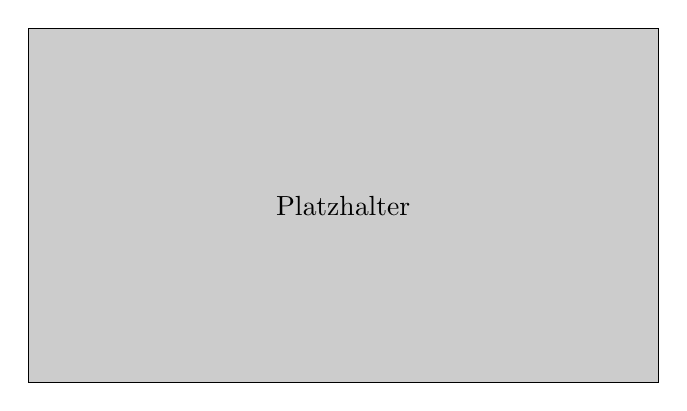
\begin{tikzpicture}
        \filldraw[fill=white!80!black,draw=black] (0,0) rectangle (8,4.5) node[pos=.5] {Platzhalter};
    \end{tikzpicture}
    \caption{Folgeregelung mit Vorsteuerung}
    \label{fig:7-11}
\end{figure}

In der Mehrzahl der Fälle haben die Regelstrecken in solchen Folgeregelungen integrierendes Verhalten mit Verzögerung (\(IT_1\)- bzw. \(IT_n\)-Verhalten).
Daher muss das Aufschaltgerät i. Allg. mehrfach differenzieren und eine Stellgröße erzeugen, die aus einer gewichteten Summe von Ableitungen der Führungsgröße nach der Zeit besteht.
Wegen gerätetechnischer Schwierigkeiten und weil höherfrequente Signalanteile durch die Differentiation stark angehoben werden, muss man sich meist auf sehr wenige Ableitungen beschränken und auf eine vollständige Kompensation dynamischer Fehler verzichten.

Bei Folgeregelungen, die im Voraus bekannte Führungsgrößenverläufe verarbeiten, wie z. B. Kopiereinrichtungen oder Vorschubeinrichtungen an numerisch gesteuerten Werkzeugmaschinen, kann man häufig die zur Vorsteuerung notwendigen Ableitungen des Führungsgrößenverlaufs analytisch oder auf anderem Wege im Voraus bestimmen.
Das kann dazu führen, dass der Folgeregelung außer dem Verlauf der Führungsgröße selbst noch die Veräufe ihrer Ableitungen nach der Zeit vorgegeben werden können.
Das Aufschaltgerät hat in diesem Fall nur eine der Regelstrecke entsprechende Gewichtung der vorgegebenen Ableitungen durchzuführen.

Al Beispiel möge ein numerisch gesteuerter Vorschubantrieb (Bild \ref{fig:7-12}) dienen, dessen dynamische Eigenschaften einem \(IT_1\)-Glied entsprechen sollen.
Für das Aufschaltgerät gilt daher
\begin{equation}
    G_A 0 \frac{1}{G_S} = \frac{1}{\frac{K_I}{s\parentheses*{1 + sT}}} = \frac{1}{K_I}s\parentheses*{1 + sT}
\end{equation}
bzw. im Zeitbereich
\begin{equation}
    y_A = \frac{1}{K_I}\parentheses*{\dot{w} + T\ddot{w}}.
\end{equation}

\begin{figure}[ht]
    \centering
    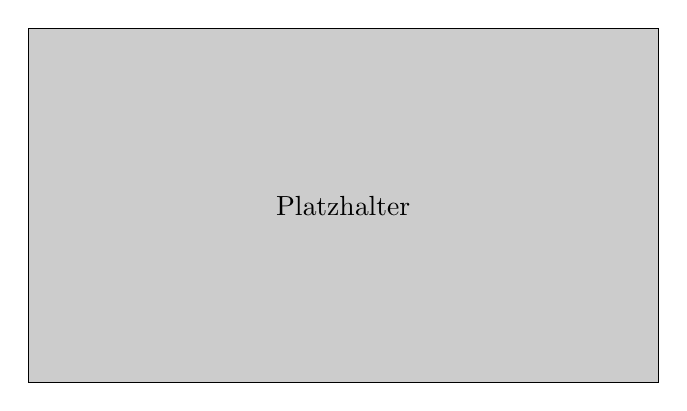
\begin{tikzpicture}
        \filldraw[fill=white!80!black,draw=black] (0,0) rectangle (8,4.5) node[pos=.5] {Platzhalter};
    \end{tikzpicture}
    \caption{Folgeregelung mit Aufschaltung der Ableitungen der Führungsgröße}
    \label{fig:7-12}
\end{figure}

Als Alternative zu der in Bild \ref{fig:7-11} dargestellten Struktur der Vorsteuerung wird die Regelung mit Führungsgrößenfilter nach Bild \ref{fig:7-13} häufig benutzt.

\begin{figure}[ht]
    \centering
    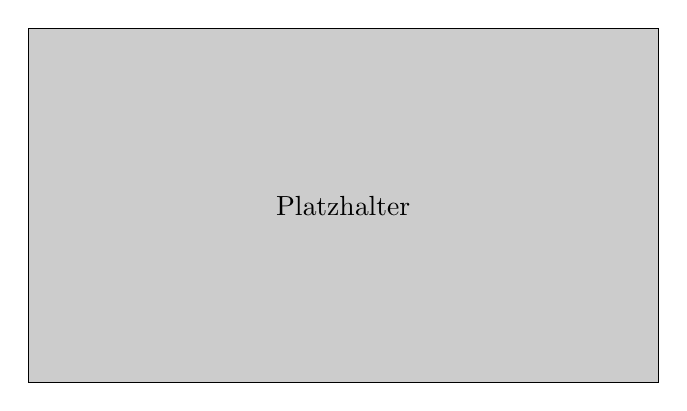
\begin{tikzpicture}
        \filldraw[fill=white!80!black,draw=black] (0,0) rectangle (8,4.5) node[pos=.5] {Platzhalter};
    \end{tikzpicture}
    \caption{Folgeregelung mit Führungsgrößenfilter}
    \label{fig:7-13}
\end{figure}

Das Führungsverhalten der Folgeregelung mit Führungsgrößenfilter (Bild \ref{fig:7-13}) wird durch die Übertragungsfunktion
\begin{equation}
    G_W = \frac{G_F G_R G_S}{1 + G_R G_S}
\end{equation}
beschrieben.
Durch Vergleich mit Gl.~\eqref{eq:7-5} erkennt man, dass die Vorsteuerung (Bild \ref{fig:7-11}) und das Führungsgrößenfilter (Bild \ref{fig:7-13}) gleich sind, wenn
\begin{equation}
    G_A + G_R = G_F \cdot G_R
\end{equation}
und damit
\begin{equation}
    \frac{G_A}{G_R} + 1 = G_F
\end{equation}
ist.
Bei der Auslegung solcher Regelungen kann der Regler mit Rücksicht auf das Störverhalten ausgelegt werden und durch das Führungsgrößenfilter kann dem Regelkreis ein gewünschtes Führungsverhalten gegeben werden.


\subsection{Mehrgrößenregelungen}

Größere Anlagen enthalten oft mehrere Regelgrößen, die durch zugeordnete Regler ihren Führungsgrößen nachgeführt bzw. angeglichen werden.
Die so entstehenden Einzelregelkreise sind häufig durch die Regelstrecken miteinander gekoppelt, d. h. eine Führungsgrößenänderung in einem der Regelkreise wirkt auf einen oder mehrere andere wie eine Störung.
Die Reaktion der Regelkreise auf die Störungen beeinflusst benachbarte Regelkreise so, dass sich zwischen den Regelkreisen geschlossene Wirkungsabläufe einstellen können, die das Gesamtsystem instabil werden lassen, obgleich jeder Teilregelkreis für sich betrachtet stabil ist.
In der regelungstechnischen Praxis treten oft sehr unübersichtliche Mehrfach- oder Mehrgrößenregelungen auf.
Es gibt eine umfassende Theorie gesteuerter und geregelter dynamischer Systeme, die auf der Beschreibung dieser Systeme mit Zustandsgrößen beruht (s. a. Kap. 8) und die Analyse und Synthese von Mehrgrößenregelungen einschließt.
Wegen des mit der Anwendung verbundenen Aufwandes wird in der Regelungspraxis meist zunächst versucht, mit den für einschleifige Regelungen gültigen Hilfsmitteln auszukommen oder diese durch einige Zusatzüberlegungen und Faustformeln zu ergänzen.

Hier sollen zunächst die zusätzlichen Probleme dargestellt werden, die aus der Kopplung mehrerer Regelkreise erwachsen.
Dies soll der Einfachheit halber nur an Zweigrößenregelungen geschehen.
Als Beispiel soll die gleichzeitige Regelung von Mischungstemperatur und Gesamtstrom in einer Flüssigkeitsmischstation betrachtet werden, die in Bild \ref{fig:7-14} schematisch wiedergegeben ist.

\begin{figure}[ht]
    \centering
    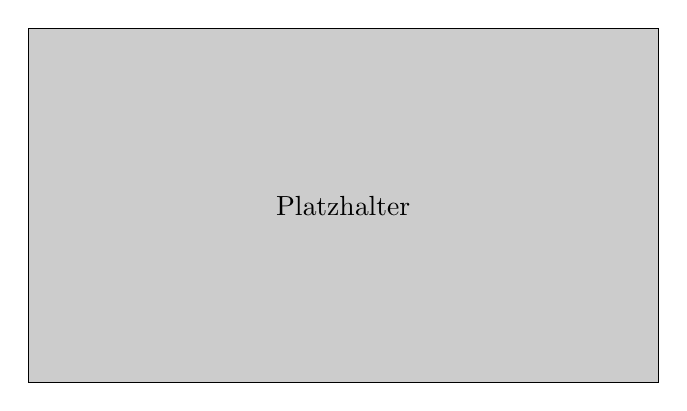
\begin{tikzpicture}
        \filldraw[fill=white!80!black,draw=black] (0,0) rectangle (8,4.5) node[pos=.5] {Platzhalter};
    \end{tikzpicture}
    \caption{Regelung von Temperatur und Durchfluss bei Mischung}
    \label{fig:7-14}
\end{figure}

Wie Bild \ref{fig:7-14} zeigt, soll die Temperatur der Mischung über den Regler \(R_{11}\) durch Verstellen des Ventils für den Zulauf warmer Flüssigkeit und der Druchfluss bzw. Mengenstrom der Mischung über den Regler \(R_{22}\) durch Verstellen des Ventils für den Zulauf kalter Flüssigkeit geregelt werden, um Störungen auszugleichen, die durch Schwankungen der Drücke \(z_1\) und \(z_2\) hervorgerufen werden.
Bild \ref{fig:7-15} zeigt den zugehörigen Wirkungsplan.

\begin{figure}[ht]
    \centering
    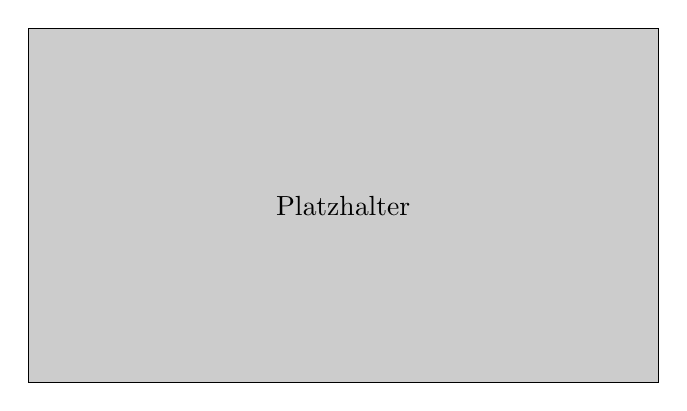
\begin{tikzpicture}
        \filldraw[fill=white!80!black,draw=black] (0,0) rectangle (8,4.5) node[pos=.5] {Platzhalter};
    \end{tikzpicture}
    \caption{Zweigrößen-Regelung mit Entkopplungsreglern}
    \label{fig:7-15}
\end{figure}

Die beiden Hauptregelkreise für Temperatur und Mengenstrom sind miteinander über die sog. Koppelstrecken \(S_{12}\) und \(S_{21}\) verbunden.
Bild \ref{fig:7-16} zeigt in einem aus dem Bild \ref{fig:7-15} entwickelten Wirkungsplan, dass der mit \(1\) bezeichnete Temperaturregelkreis als ein zur Regelstrecke \(S_{22}\) parallel geschaltetes System aufgefasst werden kann.
Für die Beurteilung des Zusammenwirkens beider Regelkreise ist wesentlich, ob die Ausgangsgrößen der beiden Koppelstrecken mit gleichem Vorzeichen (positive Kopplung) oder wie im vorliegenden Fall mit ungleichem Vorzeichen (negative Kopplung) auf die Regelgrößen wirken.
Im Allgemeinen wird durch positive Kopplung die Dämpfung verringert.

\begin{figure}[ht]
    \centering
    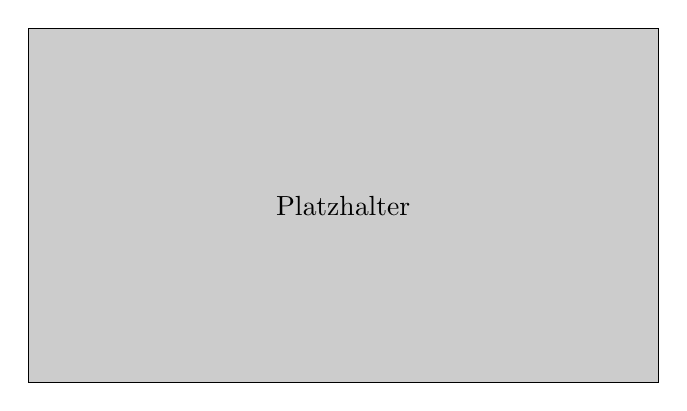
\begin{tikzpicture}
        \filldraw[fill=white!80!black,draw=black] (0,0) rectangle (8,4.5) node[pos=.5] {Platzhalter};
    \end{tikzpicture}
    \caption{Angekoppelter Regelkreis als Parallelzweig einer Regelstrecke}
    \label{fig:7-16}
\end{figure}

Der Frequenzgang der Parallelschaltung von Regelstrecke \(S_{22}\) und Regelkreis \(1\) in Bild \ref{fig:7-16} errechnet sich zu
\begin{equation}
    S_2 = \frac{\underline{x}_2}{\underline{y}_2} = S_{22} + S_{12}S_{21} \cdot \frac{R_{11}}{1 + S_{11}R_{11}}.
\end{equation}
Daran ist abzulesen, dass zumindest für niedrige Frequenzen der resultierende Frequenzgang \(S_2\) größer ist als \(S_{22}\).
Bei Systemen mit positiver Kopplung steht anstelle des Plus- ein Minuszeichen, und \(S_2\) is für niedrige Frequenzen kleiner als \(S_{22}\).
In besonders ungünstigen Fällen kann \(S_2\) zu null werden, was bedeutet, dass durch die Kopplung die Regelgröße \(x_2\) durch die Stellgröße \(y_2\) nicht mehr beeinflusst werden kann.

Damit wird deutlich, dass die bei positiver Kopplung meist zu erwartende Vergrößerung der Dämpfung des betrachteten Regelkreises mit einem Verlust an Regelwirksamkeit verbunden ist.

Die Auswirkungen unerwünschter Kopplungen kann man häufig durch den Einsatz zusätzlicher, Entkopplungsregler genannter, Übertragungsglieder vermindern.
Ziel einer solchen Entkopplung (Autonomisierung) ist, anstelle eines gekoppelten Mehrgrößensystems mehrere voneinander unabhängige Eingrößensysteme zu erhalten.
Dieses Ziel ist vollständig kaum zu erreichen, sodass man sich mit Maßnahmen begnügen muss, die Autonomie (Entkopplung) im Hinblick auf bestimmte Eingangsgrößen, z. B. Führungs- oder Störautonomie oder aber sog. Eigenautonomie (Entkopplung des aufgeschnittenen Systems) herbeiführen.
Wenn man die durch Kopplungsglieder in einen Regelkreis eingebrachten Einflüsse als Störungen definiert, dann kann man solche Entkopplungsmaßnahmen als Störgrößenaufschaltungen auffassen.

Bei der relativ einfachen Struktur des Bildes \ref{fig:7-15} lässt sich mit den angegebenen Entkopplungsreglern \(R_{12}\) und \(R_{21}\) Führungs- und Eigenautonomie zugleich erreichen, wenn man sie so auslegen kann, dass Änderungen von \(x_{w1}\) nur auf \(x_1\) und solche von \(x_{w2}\) nur auf \(x_2\) wirken.
Die Frequenzgänge der Entkopplungsregler gewinnt man z. B. aus
\begin{equation}
    \begin{split}
        -R_{11}S_{21} + R_{21}S_{22} &= 0,\\
        R_{22}S_{12} - R_{12}S_{11} &= 0
    \end{split}
\end{equation}
zu
\begin{equation}\label{eq:7-14}
    \begin{split}
        R_{21} &= R_{11} \cdot \frac{S_{21}}{S_{22}},\\
        R_{21} &= R_{22} \cdot \frac{S_{12}}{S_{11}}.
    \end{split}
\end{equation}
Ob eine vollständige Entkopplung überhaupt zu verwirklichen ist, hängt im Wesentlichen von den Frequenzgängen \(S_{22}\) und \(S_{11}\) ab, die im Nenner der Ausdrücke Gl.~\eqref{eq:7-14} stehen.
Zu Schwierigkeiten führen Glieder mit Verzögerung höherer Ordnung und besonders solche mit Totzeit- oder Allpassanteilen.
Oft begnügt man sich mit näherungsweiser oder auch mit statischer Entkopplung; bei statischer Entkopplung gelten die Ausdrücke für die Entkopplungsregler nur für die Frequenz null.
